\chapter{Technology and method}
\lhead{\emph{Technology and method}}

\section{Introduction}
% Var vi limited til å følge matistikk?
In this chapter the technology and methods applied in this project is reasoned. The project was at no point limited to follow Matistikk, but for the sake of simplicity and engineering flexibility tools which both provided good results in short time and if it were to be implemented in Matistikk, a Python solution was preferable. In addition to specific choice of tools we will also discuss th
% TODO Sjekk om jeg ikke prater opp igjen mange ganger

\section{Technology} % syns denne kan eksistere fint her

\subsection{Version control}
Throughout this project git has been used as version control. The nature of the project made us choose github as the git server, this is to easily display and share code with other people interested in the code created during the project.  

\subsection{Collaboration tools}
When collaboration tools were chosen the focus was on finding the best tool for the situation.

\subsubsection{Writing}
A decision was made on using \LaTeX as document preparation system, luckily they also have some of the best collaboration tools out there, ShareLatex. \LaTeX makes the work done stand out in a professional and clean way, it is easy to extend to fulfill needs.

\subsubsection{Storage and Mail}
For storage and mail Office365 was used (OneDrive and Outlook), this is a tool provided by NTNU for it's students. This platform enables us to easily communicate with our product owners and mentor in addition to storing our project documents and attachments.

\subsubsection{IDE/Code editor}
As an IDE/code editor we choose to partially use Visual Studio Code and Pycharm Community. One of the participants finds Pycharms debugging capabilities to be better than what Visual Studio Code could offer. After quite a while on using two different IDEs in the project we got access to Visual Studio Code live coding functionality, making it the superior tool in the last phase of our project.

\section{Python and frameworks}
The choice of technology was highly influenced by the nature of the project assignment, if the goal was to create a module for an existing Django application, Python was already the obvious choice. Eventually the project drifted in the way of a proof of concept, Python came out even further as the obvious choice. The reason why Python is the obvious choice in this case, is the ability to go from idea to a working prototype in the fastest way possible. In addition to productivity Python has a lot of mature libraries, in the nature of working towards a proof of concept, one would need stable, tested and well documented libraries. We found especially Keras \parencite{chollet_keras_2015} to be a perfect fit for our task, which is a library that makes TensorFlow or some other machine learning library easier to use.\\
\quad
The choice of back end and processing tool was now chosen, Keras backed by TensorFlow is an extremely feature-rich combination. Since the project went in the way of a proof of concept we needed some graphical user interface in which we could collect data, present statistics and so forth. The selection of front end was determined by the project assignment. Since Matistikk is web-based, we found it quite natural to go with some simple HTML, Css, JavaScript and Tornado. Tornado is a simple library to build web servers in Python.

\section{Communication and dataflow}
The foundation was quickly made, that led to an classic client/server approach. Already in the first weeks of the project Keras and deep learning was our focus.% dårlig setning...
The progress made was not only based on our own experimentation. Articles and projects posted was quickly digested and learned from. CROHME gave the project it's desirable data and insight into the assignment. CROHME provided both tools and  sequential data in InkML files, see listing \ref{lst:InkML_ex} for an InkML example file.\\
Even with the new discovered data, the research still continued.  Lu and Mohan \cite{lu_recognition_2015} and Thoma \cite{thoma_-line_2015} inspired the work made in this project. The majority of data at that stage was sequential, a decision was made to use a \gls{WebSocket} to handle front to back end communication. For the sake of simplicity, it was also implemented a way to do this over a simple http post request as an alternative to the WebSocket implementation. Doing it this way created a simple, but solid foundation for the engineers behind Matistikk to do it the way they wanted. \\
After discussion with our project owners, we were drawn to the direction of using a http post request. The test application also does not think about the amount of data it sends per classification request. If the canvas is changed, it still re-sends the entire buffer. This is both to easy re-evaluate the buffer, but in addition this can trigger changes in the segmentation process, which can eventually lead to a different classification.
%\section{Method}

%\subsection{Research}

\section{Preparing data}

\subsection{InkML}

\subsection{Images}
When deciding on the image format it was clear that the best approach was to resemble an already existing data set in order to obtain more data. Experimenting on the MNIST data made the project engineers explore possibilities to convert our InkML data to grey scale images in the same format as MNIST data. This, of course was no straight forward procedure, after several tries over a couple of weeks it was decided to go forward with generating bitmaps. Generating BMPs was a much simpler task, and luckily we found BMPs that were of handwritten mathematical symbols.

\subsubsection{Preprocessing}

This section will go through the process from when each symbol was segmented, to how the symbols were sent as input to out neural network.

The coordinates received from InkML and our own frontend application included coordinates at different scales. Therefore the traces had to be normalized, where we chose to scale traces within the range $[-1, 1]$, while still keeping the same proportions.

An example of a trace received from InkML can be seen in \ref{fig:sqrt_not_processed}.
\begin{figure}[H]
    \centering
    \includegraphics[width=\linewidth,keepaspectratio]{Assets/Chapter3_Method/sqrt_before_preprocessing.png}
    \caption{A square root which has not been through preprocessing.}
    \label{fig:sqrt_not_processed}
\end{figure}

The traces were recorded with different sampling frequencies. Some traces included several hundred points per symbol, while others included less than ten points per symbol. In order to improve performance of our network, and make the input data normalized, we reduced the number of data points per symbol through a variant of the Ramer-Douglas-Peucker algorithm \ref{ramer_douglas_peucker}. We chose to reduce all symbols to a maximum of 40 data points, if the original tracing had less than 40 data points, we padded using leading zeros. An example of the resulting trace which was used as input to our RNN can be seen below.

\begin{figure}[H]
    \centering
    \includegraphics[width=\linewidth,keepaspectratio]{Assets/Chapter3_Method/sqrt_after_preprocessing.png}
    \caption{A square root which has been through preprocessing.}
    \label{fig:sqrt_processed}
\end{figure}

To prepare trace data for the convolutional neural network, the traces were converted into an image. In order to turn traces into an image, the traces were first scaled by applying the the same scaling as previously \textbf{TODO: Ref to theory when written}, however within the range $[0, 26]$.

The next step was to generate an empty black image with 26x26 pixels (matrix of size 26x26 with only zeros). Afterwards, the pixels between each consecutive coordinate-pair were filled with white (255), and the resulting pixel grid was then normalized by dividing with 255. An example of the resulting grid presented as a matrix can be seen below, the example is simplified by using only a 8x10 matrix.

\begin{figure}[H]
    \begin{center}
    $
    \begin{bmatrix} % Jobbe mer forklaringen, vi scaler ikke 26x26 til 4x4 (?)
        \textcolor{gray}{0} & \textcolor{gray}{0} & \textcolor{gray}{0} & \textcolor{gray}{0} & \textcolor{gray}{0} & \textcolor{gray}{0} & \textcolor{gray}{0} & \textcolor{gray}{0} & \textcolor{gray}{0} & \textcolor{gray}{0} \\
        \textcolor{gray}{0} & \textcolor{gray}{0} & \textcolor{gray}{0} & \textcolor{gray}{0} & 1 & 1 & 1 & 1 & 1 & \textcolor{gray}{0} \\
        \textcolor{gray}{0} & \textcolor{gray}{0} & \textcolor{gray}{0} & 1 & \textcolor{gray}{0} & \textcolor{gray}{0} & \textcolor{gray}{0} & \textcolor{gray}{0} & \textcolor{gray}{0} & 1 \\
        1 & \textcolor{gray}{0} & \textcolor{gray}{0} & 1 & \textcolor{gray}{0} & \textcolor{gray}{0} & \textcolor{gray}{0} & \textcolor{gray}{0} & \textcolor{gray}{0} & \textcolor{gray}{0} \\
        \textcolor{gray}{0} & 1 & \textcolor{gray}{0} & 1 & \textcolor{gray}{0} & \textcolor{gray}{0} & \textcolor{gray}{0} & \textcolor{gray}{0} & \textcolor{gray}{0} & \textcolor{gray}{0} \\
        \textcolor{gray}{0} & 1 & \textcolor{gray}{0} & 1 & \textcolor{gray}{0} & \textcolor{gray}{0} & \textcolor{gray}{0} & \textcolor{gray}{0} & \textcolor{gray}{0} & \textcolor{gray}{0} \\
        \textcolor{gray}{0} & 1 & \textcolor{gray}{0} & 1 & \textcolor{gray}{0} & \textcolor{gray}{0} & \textcolor{gray}{0} & \textcolor{gray}{0} & \textcolor{gray}{0} & \textcolor{gray}{0} \\
        \textcolor{gray}{0} & \textcolor{gray}{0} & 1 & \textcolor{gray}{0} & \textcolor{gray}{0} & \textcolor{gray}{0} & \textcolor{gray}{0} & \textcolor{gray}{0} & \textcolor{gray}{0} & \textcolor{gray}{0} \\

    \end{bmatrix}
    $
    \end{center}
    \caption{A 8x10 matrix representing a pixel grid of a square root symbol.}
    \label{fig:sqrt_matrix}
\end{figure}



\begin{figure}[H]
    \centering
    \includegraphics[width=\linewidth,keepaspectratio]{Assets/Chapter3_Method/sqrt_image.png}
    \caption{The resulting square root from the preprocessing done in previous steps.\\The generated image is 26x26 pixels.}
    \label{fig:sqrt_img}
\end{figure}




\section{The recognition system}
The recognition system consists of both some "hard-coded" logic and the neural network. As stated in chapter 2.1, handwriting recognition includes several steps required to classify correctly. The "hard-coded" logic solves the segmentation issue in an elementary way, but it is quite vulnerable to noisy input. In addition to segmentation we do a whole lot of prepossessing to make sure our actual data flowing from our front end to our back end is roughly the same size format, data type and so forth. % TODO Insert a simple diagram of our system


\subsection{Preprocessing and segmentation}
%\section{Segmentation}
Since the project initially went for a solution with a CNN, we had to separate the system into different tasks. The reason behind this is that the CNN itself, in our solution should solely work on the classification of a symbol. Since our assignment is to handle symbols and expressions, we then need to extract single symbols from multiple symbols or expressions.\\
This specific task was and is the most critical in order to get correct recognition with a CNN. If the segmentation turned out wrong, the classification would be handed bad data which makes a correct classification unlikely.\\ To solve the segmentation issue different approaches was attempted, among those were object localization and detection, with bounding boxes to easily detect symbols which consists of multiple strokes or traces. This idea of object detection was quite good and would have, if successful made the rest quite easy in comparison.\\ The attempts made on object detection was unsuccessful, we were getting results, but they were not proving to be better than solving it with a much simpler algorithm which did not require machine learning in the first place. 

[TODO] positional and proportional attributes assigned to the symbols

%This decision turned out to be very wise. Eventually new data was discovered, this was from the CROHME competitions as well, but it had been turned into images for us.% CITE KAGGLE CROHME => BILDER

\subsection{Classification}

\subsubsection{Artificial Neural Network}
Artificial neural networks in image recognition is often to be found in tutorials. Since the project engineers had no prior experience with artificial neural networks it was necessary to experiment with different types of neural network and data. The MNIST data set consists of handwritten digits which is available in Keras. The amount of thorough tutorials on the MNIST data set inspired the project in new aspects. At that time, there was made a decision to use CNNs to handle the recognition problem. This meant that all the sequential data must be converted into images. \\ This was a decision that turned out to work as desired, it was not a choice that led to success. But the issue was not more focused on handling segmentation and applying different techniques to obtain good accuracy. After some experimentation with CNNs, attempts at getting it done with RNNs was started. The project went into a hard period, where we were battling variable length input and at the same time we felt that our working solution would not improve. % Trenger review..

\subsection{Interpretation and context search}
%\section{Interpretation and context search} % SKRIVER LITT OM DETTE I \section{Segmentation}
% Har skrevet om at vi hardkodet segmentering, så ta det derfra. (fins i \section{Segmentation})

The interpretation system consist of a recursive search function and a set of fixed rules to determine the context of how the symbols fit together. This step receives a list of the classified symbols from the classification step as input and outputs the interpreted context in a tree based format of objects.

\begin{figure}[H]
\begin{center}
    \includegraphics[scale=0.2]{Assets/Chapter3_Method/expression.png}
\end{center}
\centering
    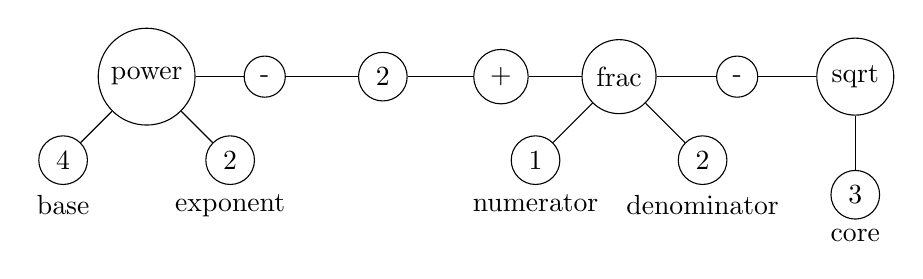
\begin{tikzpicture}[-,',auto,node distance=1.5cm,main node/.style={circle,draw}]
    \node[main node] (2) {power};
    \node[main node] (3) [right of=2] {-};
    \node[main node] (4) [right of=3] {2};
    \node[main node] (5) [right of=4] {+};
    \node[main node] (6) [right of=5] {frac};
    \node[main node] (7) [right of=6] {-};
    \node[main node] (8) [right of=7] {sqrt};
    
    \node[main node] (9) [below left of=2, label=below:base] {4};
    \node[main node] (10) [below right of=2, label=below:exponent] {2};
    
    \node[main node] (11) [below left of=6, label=below:numerator] {1};
    \node[main node] (12) [below right of=6, label=below:denominator] {2};
    
    \node[main node] (13) [below of=8, label=below:core] {3};
    
    

    \path[every node/.style={font=\sffamily\small}]
        (2) edge node [right] {} (3)
        (3) edge node [right] {} (4)
        (4) edge node [right] {} (5)
        (5) edge node [right] {} (6)
        (6) edge node [right] {} (7)
        (7) edge node [right] {} (8)
        (2) edge node [right] {} (9)
        (2) edge node [right] {} (10)
        (6) edge node [right] {} (11)
        (6) edge node [right] {} (12)
        (8) edge node [right] {} (13);

    \end{tikzpicture}
    \caption{An input expression and the resulting context tree.}

\label{fig:interpretation-tree1}
\end{figure}

% Dette kan kanskje legges i preprosessering et sted
%The symbols in the input list has a set of positional and proportional attributes that is used for sorting and to find all the symbols in an area. In addition, the attributes are used by the fixed rules to determine the notation used(see section frac-exp).

%[image of attributes on 2-3 symbols]

The system understands several mathematical notation elements, including square roots, fractions and exponents. Each of these elements has their own set of grammatical or positional rules that is used to find them (explained in section \ref{interpretation-square-roots} - \ref{interpretation-exponents}). In addition to these elements, some special symbols such as the equal sign and the multiplication dot is found and classified in this step (see section \ref{interpretation-special-symbols}).

\subsubsection{The main function}
% gangen i det hele
The main function in the interpretation system orchestrates the order of what element to search for. The order of elements searched for is:

\begin{enumerate}
    \setlength\itemsep{0.3em}
    \item Square roots
    \item Fractions
    \item Equal signs
    \item Multiplication dots
    \item Power groups, base and exponent
\end{enumerate}

The recursive part of this system comes from the square roots, fraction and exponents. If the body of a square root contains more than one symbol or object, the whole group is sent recursively to the main function. The same applies for the numerator and denominator found in fractions and for exponent-groups. The reason for this is to further search for context in these subgroups. For instance, fractions can have fractions as their numerator and exponents can consist of smaller expressions. 

This search process can be illustrated by a flowchart:

\begin{figure}[H]
\centering
    \begin{tikzpicture}[->,',auto,node distance=1.5cm,main node/.style={circle,draw},sub node/.style={draw}]
    \node[main node] (1) [label=above:Input] {};
    \node[sub node] (2) [below of=1] {Sqrt};
    \node[sub node] (3) [below of=2] {Frac};
    \node[sub node] (4) [below of=3] {$=$};
    \node[sub node] (5) [below of=4] {$\cdot$};
    \node[sub node] (6) [below of=5] {power};
    \node[main node] (7) [below of=6,label=below:Output] {};

    \path[every node/.style={font=\sffamily\small}]
        (1) edge node [right] {} (2)
        (2) edge node [right] {} (3)
        (3) edge node [right] {} (4)
        (4) edge node [right] {} (5)
        (5) edge node [right] {} (6)
        (6) edge node [right] {} (7)
        
        (2) edge[bend right=80] node [left] {core} (1)
        (3) edge[bend left=90] node [left] {numerator/denominator} (1)
        (6) edge[bend right=90] node [left] {exponent} (1);

    \end{tikzpicture}
    \caption{Flowchart of the order and recursion.}

\label{fig:interpretation_flowchart}
\end{figure}

To find the contents of a body (numerators, denominators, square root cores), the interpretation system uses the positional values of the input symbols to check whether they are inside the bounds of an area or not. If their middle point is inside this area, they are added to the output group of the area search. This area is limited by a set of maximum and minimum x- and y-coordinates. These limits comes from a set of parameters required by the main function and the positional values of control units (square roots, fraction bars).

If a square root-, fraction- or exponent-element is found, the system creates an object of the correct type and links the relevant symbols to it. When creating one of these objects the traces for each of the input symbols are combined and new positional and proportional attributes are found.

Details about how these elements are found is described in the next sections.

\subsubsection{Square roots}
\label{interpretation-square-roots}
% detaljer om kvadratrot

The square root symbols are found by creating a list of all the input symbols classified as a square root sign, by filtering out all others. These are then sorted by width to make sure that the recursive logic is maintained when searching for the bodies. The widest one is most likely the outermost one if there are roots within roots. To find the bodies the system searches for objects within the bounds specified by the positional attributes of a square root. The widest square root is evaluated first

\begin{figure}[H]
\centering
    \begin{tikzpicture}
        \node[anchor=south west,inner sep=0, scale=0.5] at (0,0) {\includegraphics[width=\textwidth]{Assets/Chapter3_Method/interpretation-sqrt.png}};
        \draw[red, thick] (1.2,0.6) rectangle (6.7,2.8);
        \draw[blue, thick] (4.7,0.8) rectangle (6.3,2.3);
    \end{tikzpicture}
    \label{fig:interpretation}
\caption{Search area of square roots.}
\end{figure}

All the symbols and objects found inside are linked to the square root object as the body. This body is then sent recursively through the main function to find the context within the square root.

\begin{figure}[H]
\begin{center}
    \includegraphics[scale=0.5]{Assets/Chapter3_Method/interpretation-sqrt.png}
\end{center}
\centering
    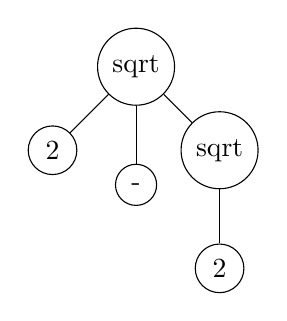
\begin{tikzpicture}[-,',auto,node distance=1.5cm,main node/.style={circle,draw}]
    \node[main node] (1) {sqrt};
    \node[main node] (2) [below left of=1] {2};
    \node[main node] (3) [below of=1] {-};
    \node[main node] (4) [below right of=1] {sqrt};
    \node[main node] (5) [below of=4] {2};
    
    

    \path[every node/.style={font=\sffamily\small}]
        (1) edge node [right] {} (2)
        (1) edge node [right] {} (3)
        (1) edge node [right] {} (4)
        (4) edge node [right] {} (5);


    \end{tikzpicture}
    \caption{An expression with a square root inside a square root and the resulting context tree.}

\label{fig:segmentation}
\end{figure}

\subsubsection{Fractions}

To find fractions the system searches for fraction bars by running the input symbols classified as minus signs through a test. To be classified as a fraction bar a minus sign must comply with one of the following cases:

\begin{itemize}
    \setlength\itemsep{0em}
    \item Have at least one symbol in the area over and under itself.
    \item Have at least two symbols in either the area over or the area under itself.
    \item Be the only minus sign in the input list and have at least one symbol in the area over or under itself.
\end{itemize}

To find the numerator and denominator of a fraction, the system searches for symbols in the area over and under the minus signs. The width of this area is specified by the leftmost and rightmost coordinate of the minus sign. The area never crosses the minus sign tested. The denominators and numerators found is also sent recursively through the main function to further look for context.

[Illustration of search area for fraction and tree, recursively]

\subsubsection{Exponents}
\label{interpretation-exponents}

Exponents are found by checking if a pair of following symbols or objects forms a power-group. A power group is the object used for base/exponent groups. To form one of these groups the exponent has to be positioned such that the following rules are complied with:

\begin{itemize}
    \setlength\itemsep{0em}
    \item The lowest point of the exponent has to be higher up than the middle y-value of the base.
    \item The middle y value of the exponent has to higher up than the upper fourth of the base.
\end{itemize}

In addition, there is a special case rule if the exponent is an operator (-, +). Then, the lowest point of the exponent has to be higher up than the upper fourth of the base.

[Illustration of rules]

The system also supports groups of symbols and objects as base or exponent. Exponents within exponents is also supported. When a base and exponent is found, the system continues to check if the next symbol also is an exponent for the same base. This search continues until a symbol conflicts with one of the rules. All the found symbols is then sent recursively through the main function again.

[illustrate steps when searching for a whole group]
[Illustration of recursion]


\subsubsection{Special case symbols}
\label{interpretation-special-symbols}

In this system there are two special case symbols: the equal sign and the multiplication dot operator. These require special treatment due to how the segmentation and classification is done. An equal sign usually consist of two traces which would be interpreted as two minus signs since the segmentation step splits them up. The multiplication sign is a small dot that, when preprocessed and scaled up, would look similar to other round symbols like 0 and $\theta$. It would therefore most likely be misclassified.

To find equal signs the system searches for minus signs that are of similar size and lined up like an equal sign. To do this, each possible pair of minus signs in the input list is tested against some rules. The pair is classified as an equal sign only if these points are fulfilled:

\begin{itemize}
    \setlength\itemsep{0em}
    \item The width of the minus signs has to be similar. The difference in width has to be less than their average width.
    \item The difference between the center x-coordinate value has to be less than a third of their combined width.
    \item The difference between the center y-coordinate value has to be less than a their average width.
\end{itemize}

These rules became such after many rounds of testing. The idea behind them was to be as general as possible.

[image of equal sign example, different varieties]

To find multiplication signs the system searches for small symbols by looking at width, height and area. Symbols are classified as multiplication signs if these rules are fulfilled:

\begin{itemize}
    \setlength\itemsep{0em}
    \item The area (height*width) of the symbol has to be less than 250.
    \item Both the height and width has to be less than 20.
    \item The height and width has to be similar. One of them cannot be more than twice the other.
\end{itemize}

These rules also went through a lot of testing to become such.

[image of multiplication sign examples]


\subsection{Converting to \LaTeX}
After the context has been found, the results can be converted to the corresponding \LaTeX code. [TODO]

\section{The project process}

The project process in terms of software engineering methodology had been a mix between multiple concepts and paradigms. In the early stages of the project methodologies from the agile world were mostly used, such as pair programming. In the early stages of the project, we followed to some extent a methodology called Lean startup. Lean startup focuses on creating a minimal viable product, often referred to as \gls{MVP}. When the MVP was out, constructive discussions with the product owners about what they liked and what they did not like. This assignment required a lot of curiosity and as project participants, one could never go hungry. This is why, at some stage the project split in different ways, we were continuously working on improving the product, but the main focus was on how we could do the recognition itself better.

\section{Teamwork and roles}
Since the project is more of a research based project, it was not easy to define a simple structure as more common in software engineering projects. Although, a simple structure was created to get the MVP up, this was Even on front end, Torkil and Håvard on back end. \\ % TODO Fortsett dette, se MAL
With the MVP up, the project quickly took principles from agile thoughts and methodologies, even though we could not plan an entire sprint to detail, we had a stand-up meeting, or quick recap of the progress and issues. This enabled a dynamic and flexible structure which led us to working together quite effective, when the project stagnated, we would quickly help each other out. When it came to exploring the potential behind RNN it was simply not easy to grasp how to approach this issue in order to classify correctly. This took one of the project engineers several weeks to get going and when the attempts were up for evaluation and the other project engineers understood the issue, a better solution and RNN was created. % Trenger kanskje ikke?

\subsection{Methodology}